% Created by tikzDevice version 0.12.3.1 on 2021-12-12 13:43:01
% !TEX encoding = UTF-8 Unicode
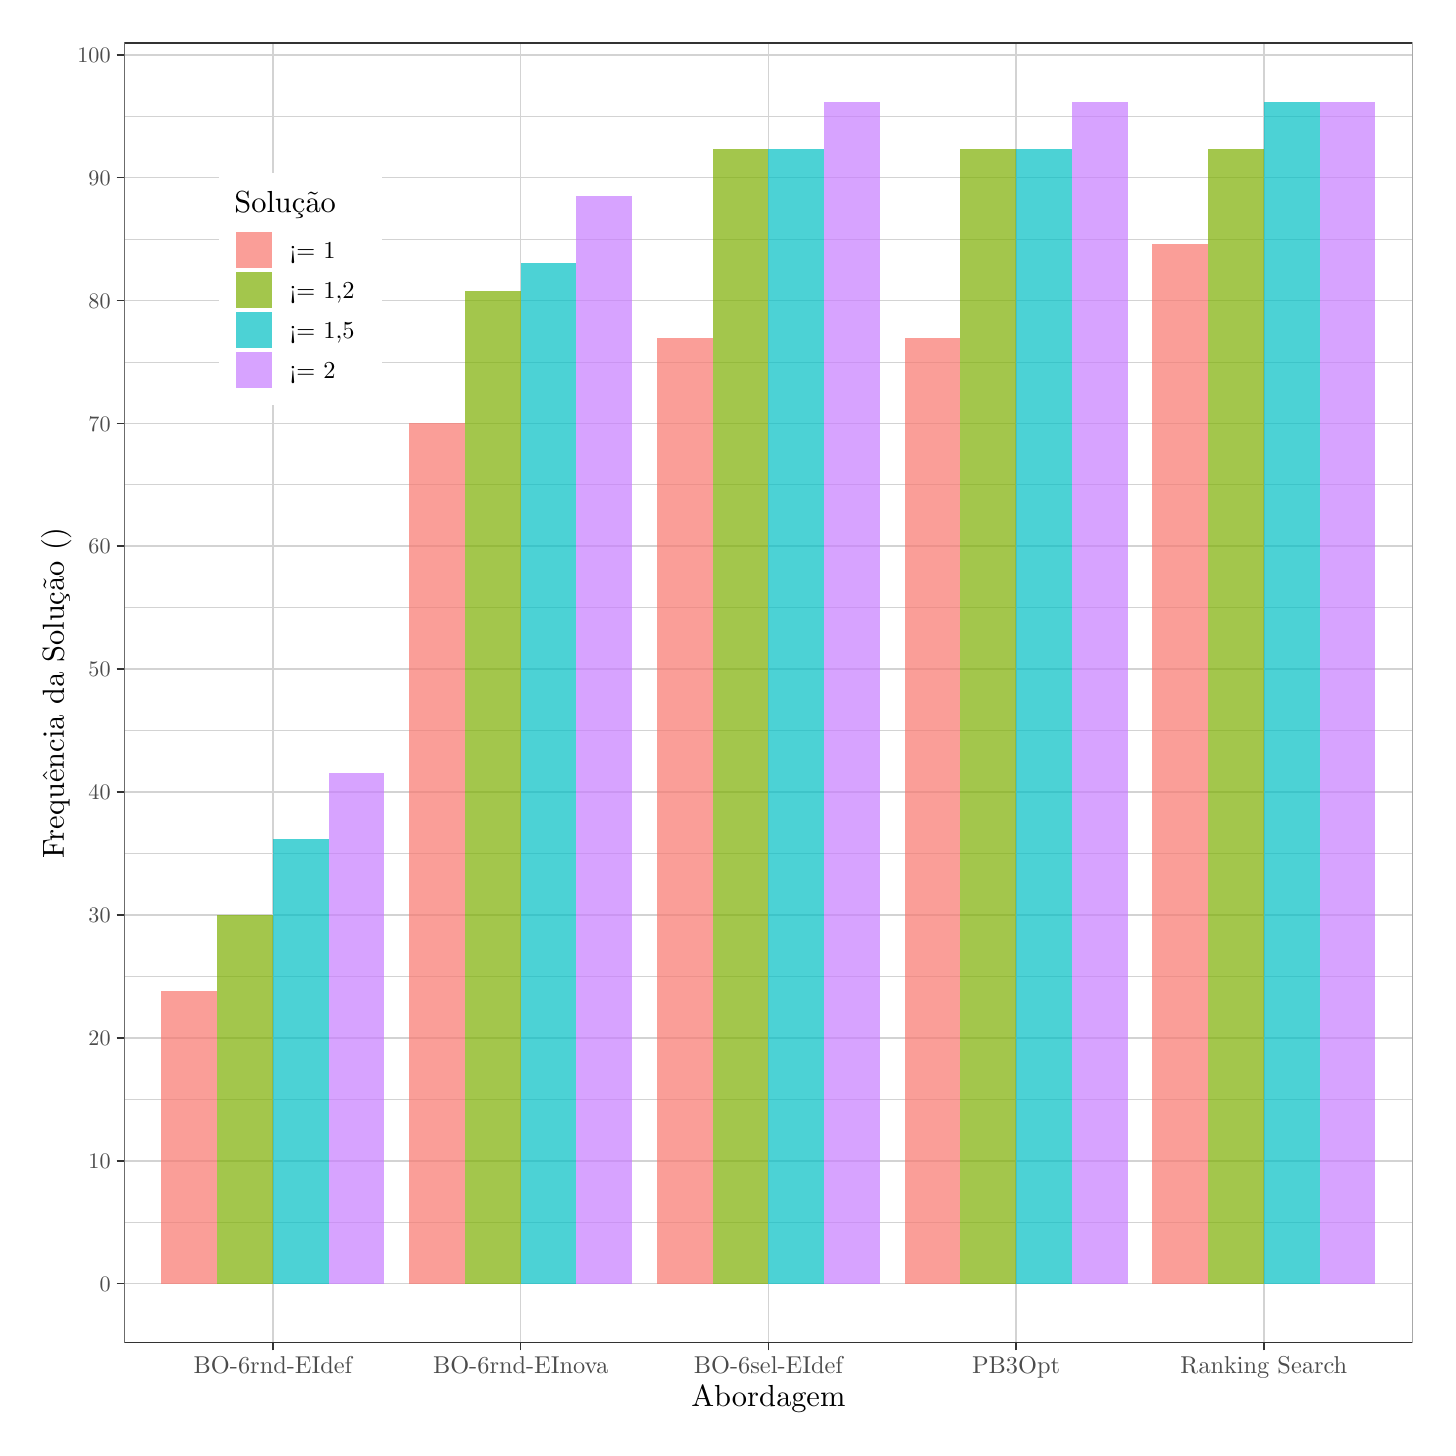
\begin{tikzpicture}[x=1pt,y=1pt]
\definecolor{fillColor}{RGB}{255,255,255}
\path[use as bounding box,fill=fillColor,fill opacity=0.00] (0,0) rectangle (505.89,505.89);
\begin{scope}
\path[clip] (  0.00,  0.00) rectangle (505.89,505.89);
\definecolor{drawColor}{RGB}{255,255,255}
\definecolor{fillColor}{RGB}{255,255,255}

\path[draw=drawColor,line width= 0.6pt,line join=round,line cap=round,fill=fillColor] (  0.00,  0.00) rectangle (505.89,505.89);
\end{scope}
\begin{scope}
\path[clip] ( 34.91, 30.69) rectangle (500.39,500.39);
\definecolor{drawColor}{RGB}{190,190,190}
\definecolor{fillColor}{RGB}{255,255,255}

\path[draw=drawColor,line width= 0.6pt,line join=round,line cap=round,fill=fillColor] ( 34.91, 30.69) rectangle (500.39,500.39);
\definecolor{drawColor}{RGB}{211,211,211}

\path[draw=drawColor,line width= 0.3pt,line join=round] ( 34.91, 74.24) --
	(500.39, 74.24);

\path[draw=drawColor,line width= 0.3pt,line join=round] ( 34.91,118.65) --
	(500.39,118.65);

\path[draw=drawColor,line width= 0.3pt,line join=round] ( 34.91,163.06) --
	(500.39,163.06);

\path[draw=drawColor,line width= 0.3pt,line join=round] ( 34.91,207.47) --
	(500.39,207.47);

\path[draw=drawColor,line width= 0.3pt,line join=round] ( 34.91,251.87) --
	(500.39,251.87);

\path[draw=drawColor,line width= 0.3pt,line join=round] ( 34.91,296.28) --
	(500.39,296.28);

\path[draw=drawColor,line width= 0.3pt,line join=round] ( 34.91,340.69) --
	(500.39,340.69);

\path[draw=drawColor,line width= 0.3pt,line join=round] ( 34.91,385.10) --
	(500.39,385.10);

\path[draw=drawColor,line width= 0.3pt,line join=round] ( 34.91,429.51) --
	(500.39,429.51);

\path[draw=drawColor,line width= 0.3pt,line join=round] ( 34.91,473.92) --
	(500.39,473.92);

\path[draw=drawColor,line width= 0.6pt,line join=round] ( 34.91, 52.04) --
	(500.39, 52.04);

\path[draw=drawColor,line width= 0.6pt,line join=round] ( 34.91, 96.44) --
	(500.39, 96.44);

\path[draw=drawColor,line width= 0.6pt,line join=round] ( 34.91,140.85) --
	(500.39,140.85);

\path[draw=drawColor,line width= 0.6pt,line join=round] ( 34.91,185.26) --
	(500.39,185.26);

\path[draw=drawColor,line width= 0.6pt,line join=round] ( 34.91,229.67) --
	(500.39,229.67);

\path[draw=drawColor,line width= 0.6pt,line join=round] ( 34.91,274.08) --
	(500.39,274.08);

\path[draw=drawColor,line width= 0.6pt,line join=round] ( 34.91,318.49) --
	(500.39,318.49);

\path[draw=drawColor,line width= 0.6pt,line join=round] ( 34.91,362.89) --
	(500.39,362.89);

\path[draw=drawColor,line width= 0.6pt,line join=round] ( 34.91,407.30) --
	(500.39,407.30);

\path[draw=drawColor,line width= 0.6pt,line join=round] ( 34.91,451.71) --
	(500.39,451.71);

\path[draw=drawColor,line width= 0.6pt,line join=round] ( 34.91,496.12) --
	(500.39,496.12);

\path[draw=drawColor,line width= 0.6pt,line join=round] ( 88.62, 30.69) --
	( 88.62,500.39);

\path[draw=drawColor,line width= 0.6pt,line join=round] (178.14, 30.69) --
	(178.14,500.39);

\path[draw=drawColor,line width= 0.6pt,line join=round] (267.65, 30.69) --
	(267.65,500.39);

\path[draw=drawColor,line width= 0.6pt,line join=round] (357.17, 30.69) --
	(357.17,500.39);

\path[draw=drawColor,line width= 0.6pt,line join=round] (446.68, 30.69) --
	(446.68,500.39);
\definecolor{fillColor}{RGB}{248,118,109}

\path[fill=fillColor,fill opacity=0.70] ( 48.34, 52.04) rectangle ( 68.48,157.93);

\path[fill=fillColor,fill opacity=0.70] (137.85, 52.04) rectangle (157.99,362.89);

\path[fill=fillColor,fill opacity=0.70] (227.37, 52.04) rectangle (247.51,393.64);

\path[fill=fillColor,fill opacity=0.70] (316.88, 52.04) rectangle (337.02,393.64);

\path[fill=fillColor,fill opacity=0.70] (406.40, 52.04) rectangle (426.54,427.80);
\definecolor{fillColor}{RGB}{124,174,0}

\path[fill=fillColor,fill opacity=0.70] ( 68.48, 52.04) rectangle ( 88.62,185.26);

\path[fill=fillColor,fill opacity=0.70] (157.99, 52.04) rectangle (178.14,410.72);

\path[fill=fillColor,fill opacity=0.70] (247.51, 52.04) rectangle (267.65,461.96);

\path[fill=fillColor,fill opacity=0.70] (337.02, 52.04) rectangle (357.17,461.96);

\path[fill=fillColor,fill opacity=0.70] (426.54, 52.04) rectangle (446.68,461.96);
\definecolor{fillColor}{RGB}{0,191,196}

\path[fill=fillColor,fill opacity=0.70] ( 88.62, 52.04) rectangle (108.76,212.59);

\path[fill=fillColor,fill opacity=0.70] (178.14, 52.04) rectangle (198.28,420.97);

\path[fill=fillColor,fill opacity=0.70] (267.65, 52.04) rectangle (287.79,461.96);

\path[fill=fillColor,fill opacity=0.70] (357.17, 52.04) rectangle (377.31,461.96);

\path[fill=fillColor,fill opacity=0.70] (446.68, 52.04) rectangle (466.82,479.04);
\definecolor{fillColor}{RGB}{199,124,255}

\path[fill=fillColor,fill opacity=0.70] (108.76, 52.04) rectangle (128.90,236.50);

\path[fill=fillColor,fill opacity=0.70] (198.28, 52.04) rectangle (218.42,444.88);

\path[fill=fillColor,fill opacity=0.70] (287.79, 52.04) rectangle (307.93,479.04);

\path[fill=fillColor,fill opacity=0.70] (377.31, 52.04) rectangle (397.45,479.04);

\path[fill=fillColor,fill opacity=0.70] (466.82, 52.04) rectangle (486.96,479.04);
\definecolor{drawColor}{gray}{0.20}

\path[draw=drawColor,line width= 0.6pt,line join=round,line cap=round] ( 34.91, 30.69) rectangle (500.39,500.39);
\end{scope}
\begin{scope}
\path[clip] (  0.00,  0.00) rectangle (505.89,505.89);
\definecolor{drawColor}{gray}{0.30}

\node[text=drawColor,anchor=base east,inner sep=0pt, outer sep=0pt, scale=  0.80] at ( 29.96, 49.28) {0};

\node[text=drawColor,anchor=base east,inner sep=0pt, outer sep=0pt, scale=  0.80] at ( 29.96, 93.69) {10};

\node[text=drawColor,anchor=base east,inner sep=0pt, outer sep=0pt, scale=  0.80] at ( 29.96,138.10) {20};

\node[text=drawColor,anchor=base east,inner sep=0pt, outer sep=0pt, scale=  0.80] at ( 29.96,182.51) {30};

\node[text=drawColor,anchor=base east,inner sep=0pt, outer sep=0pt, scale=  0.80] at ( 29.96,226.91) {40};

\node[text=drawColor,anchor=base east,inner sep=0pt, outer sep=0pt, scale=  0.80] at ( 29.96,271.32) {50};

\node[text=drawColor,anchor=base east,inner sep=0pt, outer sep=0pt, scale=  0.80] at ( 29.96,315.73) {60};

\node[text=drawColor,anchor=base east,inner sep=0pt, outer sep=0pt, scale=  0.80] at ( 29.96,360.14) {70};

\node[text=drawColor,anchor=base east,inner sep=0pt, outer sep=0pt, scale=  0.80] at ( 29.96,404.55) {80};

\node[text=drawColor,anchor=base east,inner sep=0pt, outer sep=0pt, scale=  0.80] at ( 29.96,448.96) {90};

\node[text=drawColor,anchor=base east,inner sep=0pt, outer sep=0pt, scale=  0.80] at ( 29.96,493.37) {100};
\end{scope}
\begin{scope}
\path[clip] (  0.00,  0.00) rectangle (505.89,505.89);
\definecolor{drawColor}{gray}{0.20}

\path[draw=drawColor,line width= 0.6pt,line join=round] ( 32.16, 52.04) --
	( 34.91, 52.04);

\path[draw=drawColor,line width= 0.6pt,line join=round] ( 32.16, 96.44) --
	( 34.91, 96.44);

\path[draw=drawColor,line width= 0.6pt,line join=round] ( 32.16,140.85) --
	( 34.91,140.85);

\path[draw=drawColor,line width= 0.6pt,line join=round] ( 32.16,185.26) --
	( 34.91,185.26);

\path[draw=drawColor,line width= 0.6pt,line join=round] ( 32.16,229.67) --
	( 34.91,229.67);

\path[draw=drawColor,line width= 0.6pt,line join=round] ( 32.16,274.08) --
	( 34.91,274.08);

\path[draw=drawColor,line width= 0.6pt,line join=round] ( 32.16,318.49) --
	( 34.91,318.49);

\path[draw=drawColor,line width= 0.6pt,line join=round] ( 32.16,362.89) --
	( 34.91,362.89);

\path[draw=drawColor,line width= 0.6pt,line join=round] ( 32.16,407.30) --
	( 34.91,407.30);

\path[draw=drawColor,line width= 0.6pt,line join=round] ( 32.16,451.71) --
	( 34.91,451.71);

\path[draw=drawColor,line width= 0.6pt,line join=round] ( 32.16,496.12) --
	( 34.91,496.12);
\end{scope}
\begin{scope}
\path[clip] (  0.00,  0.00) rectangle (505.89,505.89);
\definecolor{drawColor}{gray}{0.20}

\path[draw=drawColor,line width= 0.6pt,line join=round] ( 88.62, 27.94) --
	( 88.62, 30.69);

\path[draw=drawColor,line width= 0.6pt,line join=round] (178.14, 27.94) --
	(178.14, 30.69);

\path[draw=drawColor,line width= 0.6pt,line join=round] (267.65, 27.94) --
	(267.65, 30.69);

\path[draw=drawColor,line width= 0.6pt,line join=round] (357.17, 27.94) --
	(357.17, 30.69);

\path[draw=drawColor,line width= 0.6pt,line join=round] (446.68, 27.94) --
	(446.68, 30.69);
\end{scope}
\begin{scope}
\path[clip] (  0.00,  0.00) rectangle (505.89,505.89);
\definecolor{drawColor}{gray}{0.30}

\node[text=drawColor,anchor=base,inner sep=0pt, outer sep=0pt, scale=  0.88] at ( 88.62, 19.68) {BO-6rnd-EIdef};

\node[text=drawColor,anchor=base,inner sep=0pt, outer sep=0pt, scale=  0.88] at (178.14, 19.68) {BO-6rnd-EInova};

\node[text=drawColor,anchor=base,inner sep=0pt, outer sep=0pt, scale=  0.88] at (267.65, 19.68) {BO-6sel-EIdef};

\node[text=drawColor,anchor=base,inner sep=0pt, outer sep=0pt, scale=  0.88] at (357.17, 19.68) {PB3Opt};

\node[text=drawColor,anchor=base,inner sep=0pt, outer sep=0pt, scale=  0.88] at (446.68, 19.68) {Ranking Search};
\end{scope}
\begin{scope}
\path[clip] (  0.00,  0.00) rectangle (505.89,505.89);
\definecolor{drawColor}{RGB}{0,0,0}

\node[text=drawColor,anchor=base,inner sep=0pt, outer sep=0pt, scale=  1.10] at (267.65,  7.64) {Abordagem};
\end{scope}
\begin{scope}
\path[clip] (  0.00,  0.00) rectangle (505.89,505.89);
\definecolor{drawColor}{RGB}{0,0,0}

\node[text=drawColor,rotate= 90.00,anchor=base,inner sep=0pt, outer sep=0pt, scale=  1.10] at ( 13.08,265.54) {Frequência da Solução ()};
\end{scope}
\begin{scope}
\path[clip] (  0.00,  0.00) rectangle (505.89,505.89);
\definecolor{fillColor}{RGB}{255,255,255}

\path[fill=fillColor] ( 69.19,369.39) rectangle (128.01,453.42);
\end{scope}
\begin{scope}
\path[clip] (  0.00,  0.00) rectangle (505.89,505.89);
\definecolor{drawColor}{RGB}{0,0,0}

\node[text=drawColor,anchor=base west,inner sep=0pt, outer sep=0pt, scale=  1.10] at ( 74.69,439.27) {Solução};
\end{scope}
\begin{scope}
\path[clip] (  0.00,  0.00) rectangle (505.89,505.89);
\definecolor{fillColor}{RGB}{255,255,255}

\path[fill=fillColor] ( 74.69,418.25) rectangle ( 89.15,432.71);
\end{scope}
\begin{scope}
\path[clip] (  0.00,  0.00) rectangle (505.89,505.89);
\definecolor{fillColor}{RGB}{248,118,109}

\path[fill=fillColor,fill opacity=0.70] ( 75.40,418.96) rectangle ( 88.44,431.99);
\end{scope}
\begin{scope}
\path[clip] (  0.00,  0.00) rectangle (505.89,505.89);
\definecolor{fillColor}{RGB}{255,255,255}

\path[fill=fillColor] ( 74.69,403.80) rectangle ( 89.15,418.25);
\end{scope}
\begin{scope}
\path[clip] (  0.00,  0.00) rectangle (505.89,505.89);
\definecolor{fillColor}{RGB}{124,174,0}

\path[fill=fillColor,fill opacity=0.70] ( 75.40,404.51) rectangle ( 88.44,417.54);
\end{scope}
\begin{scope}
\path[clip] (  0.00,  0.00) rectangle (505.89,505.89);
\definecolor{fillColor}{RGB}{255,255,255}

\path[fill=fillColor] ( 74.69,389.34) rectangle ( 89.15,403.80);
\end{scope}
\begin{scope}
\path[clip] (  0.00,  0.00) rectangle (505.89,505.89);
\definecolor{fillColor}{RGB}{0,191,196}

\path[fill=fillColor,fill opacity=0.70] ( 75.40,390.05) rectangle ( 88.44,403.09);
\end{scope}
\begin{scope}
\path[clip] (  0.00,  0.00) rectangle (505.89,505.89);
\definecolor{fillColor}{RGB}{255,255,255}

\path[fill=fillColor] ( 74.69,374.89) rectangle ( 89.15,389.34);
\end{scope}
\begin{scope}
\path[clip] (  0.00,  0.00) rectangle (505.89,505.89);
\definecolor{fillColor}{RGB}{199,124,255}

\path[fill=fillColor,fill opacity=0.70] ( 75.40,375.60) rectangle ( 88.44,388.63);
\end{scope}
\begin{scope}
\path[clip] (  0.00,  0.00) rectangle (505.89,505.89);
\definecolor{drawColor}{RGB}{0,0,0}

\node[text=drawColor,anchor=base west,inner sep=0pt, outer sep=0pt, scale=  0.88] at ( 94.65,422.45) {<= 1};
\end{scope}
\begin{scope}
\path[clip] (  0.00,  0.00) rectangle (505.89,505.89);
\definecolor{drawColor}{RGB}{0,0,0}

\node[text=drawColor,anchor=base west,inner sep=0pt, outer sep=0pt, scale=  0.88] at ( 94.65,407.99) {<= 1,2};
\end{scope}
\begin{scope}
\path[clip] (  0.00,  0.00) rectangle (505.89,505.89);
\definecolor{drawColor}{RGB}{0,0,0}

\node[text=drawColor,anchor=base west,inner sep=0pt, outer sep=0pt, scale=  0.88] at ( 94.65,393.54) {<= 1,5};
\end{scope}
\begin{scope}
\path[clip] (  0.00,  0.00) rectangle (505.89,505.89);
\definecolor{drawColor}{RGB}{0,0,0}

\node[text=drawColor,anchor=base west,inner sep=0pt, outer sep=0pt, scale=  0.88] at ( 94.65,379.09) {<= 2};
\end{scope}
\end{tikzpicture}
